\documentclass[11pt,a4paper]{article}
\usepackage[T1]{fontenc}
\usepackage[utf8]{inputenc}
\usepackage[magyar]{babel}
\usepackage{lmodern}
\usepackage{amsmath,amssymb}
\usepackage{enumitem}
\usepackage{tikz}
\usetikzlibrary{arrows.meta}
\usepackage[a4paper,margin=2cm]{geometry}

\pagestyle{empty}
\setlength{\parindent}{0pt}
\setlist[enumerate,1]{label=\textbf{\arabic*.}, leftmargin=*, itemsep=10pt, topsep=3pt}
\setlist[enumerate,2]{label=\alph*), leftmargin=2em, itemsep=4pt, topsep=3pt, parsep=0pt}

\begin{document}

\begin{center}
  {\Large\bfseries A fény kettős természete -- gyakorló feladatok -- megoldókulcs}
\end{center}

\begin{enumerate}
\item \textbf{Hőmérsékleti sugárzás}
  \begin{enumerate}
    \item Magasabb hőmérsékleten a csúcs a \textbf{rövidebb hullámhosszak} felé tolódik:
      a test színe a vörösből a narancson át a fehér felé változik. A görbe alatti
      terület (a teljes kisugárzott teljesítmény) erősen \textbf{nő}: a
      Stefan--Boltzmann-törvény szerint $T^4$-nel arányos.
    \item Nap: $\lambda_\text{max} = \dfrac{2{,}9\cdot 10^{-3}}{5800}~\text{m} =
      5{,}0\cdot 10^{-7}~\text{m} = 500~\text{nm}$, a látható tartomány közepe.\\
      Izzószál: $\lambda_\text{max} = \dfrac{2{,}9\cdot 10^{-3}}{2800}~\text{m} \approx
      1{,}04~\mu\text{m}$, már az infravörösben van. Az izzó sugárzásának nagy része
      infravörös (hő), a láthatóba csak néhány százalék esik, ezért rossz fényforrás.
      (Kiegészítés: az emberi test $310$~K-en kb.\ $9{,}4~\mu\text{m}$-en sugároz a
      legerősebben, ezt látja a hőkamera.)
    \item $E = hf = \dfrac{hc}{\lambda} = \dfrac{6{,}63\cdot 10^{-34}\cdot 3\cdot 10^8}
      {5\cdot 10^{-7}}~\text{J} \approx 3{,}98\cdot 10^{-19}~\text{J} \approx
      2{,}5~\text{eV}$.
  \end{enumerate}

\item \textbf{Optikai rács}
  \begin{enumerate}
    \item $d = \dfrac{1~\text{mm}}{500} = 2~\mu\text{m}$. A maximumok feltétele
      $d\sin\alpha_k = k\lambda$:\\
      $\sin\alpha_1 = \dfrac{0{,}6}{2} = 0{,}3 \Rightarrow \alpha_1 \approx 17{,}5^\circ$,
      $\;x_1 = L\tan\alpha_1 \approx 31{,}4~\text{cm}$;\\
      $\sin\alpha_2 = 0{,}6 \Rightarrow \alpha_2 \approx 36{,}9^\circ$,
      $\;x_2 = L\tan\alpha_2 = 75~\text{cm}$.\\
      \emph{Tipikus hiba:} a kis szögekre érvényes $x \approx k\lambda L/d$ közelítés
      $30$ és $60$~cm-t adna. A második rendnél ez már 20\%-os hiba, itt nem
      használható.
    \item $\sin\alpha \le 1 \Rightarrow k \le d/\lambda = 3{,}33$, tehát $k_\text{max} = 3$.
      Összesen $2\cdot 3 + 1 = 7$ fényes folt ($k = 0, \pm1, \pm2, \pm3$).
    \item Bizonyos irányokban \emph{fény $+$ fény $=$ sötétség}: ott a különböző résekből
      érkező hullámok ellentétes fázisban találkoznak és kioltják egymást (destruktív
      interferencia). Részecskékkel ez nem magyarázható: ha több résen több részecske
      jut át, mindenhol csak \emph{több} fény lehetne, sötét helyek nem. A maximumok
      helyét is pontosan az útkülönbség ($d\sin\alpha = k\lambda$) adja meg.
  \end{enumerate}

\item \textbf{Fényelektromos jelenség}
  \begin{enumerate}
    \item A hullámelmélet szerint a hullám energiája az intenzitással nő. Elég erős
      (vagy elég hosszan sugárzó) lámpa bármilyen színnel előbb-utóbb elég energiát adna
      az elektronoknak a kilépéshez. A kísérletben viszont nem a fény erőssége, hanem a
      \textbf{színe (frekvenciája)} dönt, és ez a hullámképben érthetetlen.
    \item \textbf{(1) Határfrekvencia:} egy foton egyetlen elektronnak adja át a teljes
      $hf$ energiáját. Ha $hf < W_\text{ki}$, egyetlen foton sem tud elektront kiszakítani,
      akárhány foton érkezik is (két foton energiája nem adódik össze egy elektronon).
      A határ: $f_0 = W_\text{ki}/h$.\\
      \textbf{(2) Mozgási energia:} az elektron $hf$ energiát kap, ebből legalább
      $W_\text{ki}$ a kilépésre megy el, a maradék legfeljebb $hf - W_\text{ki}$: ez csak
      a frekvenciától függ. Az intenzitás a fotonok \emph{számát} adja meg, ezért a
      kilépő elektronok számát (a fotoáramot) növeli, az energiájukat nem.\\
      \textbf{(3) Nincs késés:} az energia adagokban érkezik, az elektron egyetlen
      fotont egyszerre nyel el, nem kell energiát ,,gyűjtenie''.
    \item $hf = W_\text{ki} + \tfrac12 m v_\text{max}^2$. Itt $hf$ a foton energiája,
      $W_\text{ki}$ a kilépési munka (az anyagra jellemző legkisebb energia, amely egy
      elektron kiszakításához kell), $\tfrac12 m v_\text{max}^2$ a kilépő elektronok
      legnagyobb mozgási energiája.
  \end{enumerate}
  \emph{Kimaradt kérdés, ha jut rá idő:} pozitív lemeznél UV-fénnyel sincs kisülés,
  mert a kilépő elektronokat a pozitív lemez visszavonzza. Ebből látszik, hogy a kilépő
  részecskék negatív töltésűek.

\item \textbf{Millikan mérése}
  \begin{enumerate}
    \item A fékező térben az elektronok mozgási energiája csökken: a tér $eU$ munkát
      végez ellenük. Az áram akkor szűnik meg, amikor már a leggyorsabb elektronok sem
      érik el az anódot: $eU_\text{z} = \tfrac12 m v_\text{max}^2$. Így a voltban mért
      $U_\text{z}$ éppen a legnagyobb mozgási energia eV-ban.
    \item
      \begin{minipage}[t]{0.55\linewidth}\raggedright
      $eU_\text{z} = hf - W_\text{ki} \Rightarrow U_\text{z} = \dfrac{h}{e}\,f -
      \dfrac{W_\text{ki}}{e}$: egyenes, meredeksége $h/e$.\\[3pt]
      Meredekség (illesztett egyenesből):
      $\dfrac{1{,}83 - 0{,}19}{(10-6)\cdot 10^{14}}~\tfrac{\text{V}}{\text{Hz}}
      \approx 4{,}1\cdot 10^{-15}~\text{V}\cdot\text{s}$, így
      $h = e\cdot 4{,}1\cdot 10^{-15} \approx 6{,}6\cdot 10^{-34}~\text{J}\cdot\text{s}$.\\[3pt]
      Az $f$ tengellyel való metszéspont: $f_0 \approx 5{,}5\cdot 10^{14}~\text{Hz}$.\\
      $W_\text{ki} = hf_0 \approx 2{,}3~\text{eV}$ (az egyenes $f = 0$-nál $-2{,}3$~V-nál
      metszené a függőleges tengelyt). Ez a nátrium kilépési munkája.\\
      $\lambda_0 = c/f_0 \approx 540~\text{nm}$ (zöld): vörös vagy sárga fény ebből a
      katódból nem vált ki elektront.\\[3pt]
      \emph{Elfogadható tartomány} (grafikus leolvasásnál):
      $h \approx (6{,}3$--$6{,}9)\cdot 10^{-34}~\text{J}\cdot\text{s}$,
      $W_\text{ki} \approx 2{,}2$--$2{,}4$~eV.
      \end{minipage}\hfill
      \begin{minipage}[t]{0.42\linewidth}\vspace{0pt}\centering
      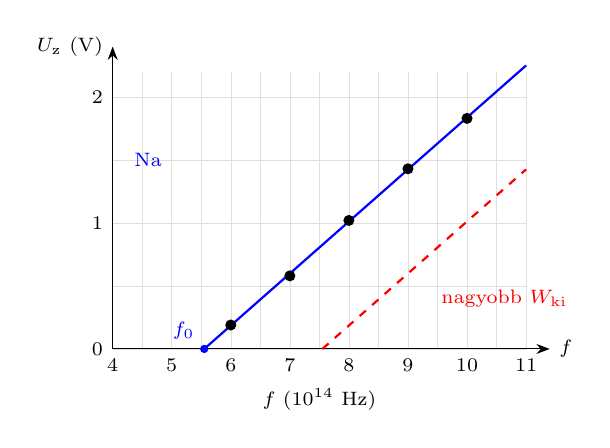
\begin{tikzpicture}[x=0.75cm,y=1.6cm,>=Stealth]
        \draw[step=0.5,gray!25,very thin] (0,0) grid (7,2.2);
        \draw[->] (0,0) -- (7.4,0) node[right] {\scriptsize $f$};
        \draw[->] (0,0) -- (0,2.4) node[left] {\scriptsize $U_\text{z}$ (V)};
        \foreach \x/\l in {0/4,1/5,2/6,3/7,4/8,5/9,6/10,7/11}
          \node[below,font=\scriptsize] at (\x,0) {\l};
        \foreach \y in {0,1,2} \node[left,font=\scriptsize] at (0,\y) {\y};
        \node[font=\scriptsize] at (3.5,-0.4) {$f$ ($10^{14}$ Hz)};
        \draw[thick,blue] (1.55,0) -- (7,2.25);
        \draw[thick,red,dashed] (3.55,0) -- (7,1.425);
        \foreach \x/\y in {2/0.19,3/0.58,4/1.02,5/1.43,6/1.83}
          \fill (\x,\y) circle (2pt);
        \node[blue,font=\scriptsize,anchor=west] at (0.2,1.5) {Na};
        \node[red,font=\scriptsize,anchor=west] at (5.4,0.4) {nagyobb $W_\text{ki}$};
        \fill[blue] (1.55,0) circle (1.5pt) node[above left,font=\scriptsize] {$f_0$};
      \end{tikzpicture}
      \end{minipage}
    \item $f = c/\lambda = 7{,}5\cdot 10^{14}~\text{Hz}$, $\;hf \approx 4{,}97\cdot
      10^{-19}~\text{J} \approx 3{,}1~\text{eV}$.\\
      $E_\text{max} = 3{,}1 - 2{,}3 = 0{,}8~\text{eV} \approx 1{,}3\cdot 10^{-19}~\text{J}$
      (a grafikonról is leolvasható: $U_\text{z} \approx 0{,}8$~V).\\
      $v_\text{max} = \sqrt{2E_\text{max}/m} = \sqrt{\dfrac{2\cdot 1{,}3\cdot 10^{-19}}
      {9{,}1\cdot 10^{-31}}}~\tfrac{\text{m}}{\text{s}} \approx
      5{,}3\cdot 10^{5}~\tfrac{\text{m}}{\text{s}}$.
    \item \textbf{Kétszeres intenzitás:} a grafikon \emph{nem változik}, mert
      $U_\text{z}$ csak $f$-től függ; csak a fotoáram lesz kétszeres.\\
      \textbf{Nagyobb kilépési munka:} \emph{párhuzamos} egyenes, jobbra tolva (nagyobb
      $f_0$). A meredekség ($h/e$) minden fémre ugyanaz: $h$ természeti állandó, nem
      anyagjellemző.
  \end{enumerate}

\item \textbf{De Broglie-hullámok}
  \begin{enumerate}
    \item $E = eU = 1{,}6\cdot 10^{-17}~\text{J}$, $\;p = \sqrt{2mE} =
      \sqrt{2\cdot 9{,}1\cdot 10^{-31}\cdot 1{,}6\cdot 10^{-17}} \approx
      5{,}4\cdot 10^{-24}~\tfrac{\text{kg}\cdot\text{m}}{\text{s}}$.\\
      $\lambda = h/p \approx 1{,}2\cdot 10^{-10}~\text{m} = 0{,}12~\text{nm}$.\\
      Ez akkora, mint az atomok távolsága a kristályban, ezért a kristályrács
      \textbf{elhajlási rácsként} működik az elektronokra (Davisson--Germer, 1927: az
      elektronelhajlás kísérleti bizonyítéka). Egy optikai rács rácsállandója
      ($\sim\mu\text{m}$) tízezerszer nagyobb, ezért $\sin\alpha = \lambda/d \sim
      10^{-4}$: az elhajlás szöge mérhetetlenül kicsi lenne.
    \item $p = 0{,}06\cdot 30 = 1{,}8~\tfrac{\text{kg}\cdot\text{m}}{\text{s}}$,
      $\;\lambda = \dfrac{6{,}63\cdot 10^{-34}}{1{,}8}~\text{m} \approx
      3{,}7\cdot 10^{-34}~\text{m}$. Ez sok nagyságrenddel kisebb egy atommagnál is
      ($\sim 10^{-15}$~m). Nincs olyan rés vagy akadály, amelyen ez kimutatható lenne,
      ezért makroszkopikus testeknél a hullámtermészet nem észlelhető.
    \item \textbf{Egy becsapódás:} egyetlen pontban, ,,egészben'' érkezik az elektron
      (részecskeként), és a helye előre nem jósolható meg, véletlenszerű.
      \textbf{Sok becsapódás:} kirajzolódik a kétréses interferenciakép. A becsapódások
      eloszlását a hullám írja le.\\
      Értelmezés: a hullám (pontosabban az amplitúdó négyzete) azt adja meg, mekkora
      \textbf{valószínűséggel} találjuk az elektront egy adott helyen. Mivel az
      elektronokat egyenként küldtük, az interferencia nem az elektronok egymásra
      hatásából jön: minden egyes elektron hullámként mindkét résen ,,átmegy''. Nagyon
      gyenge fénnyel (egyenként érkező fotonokkal) pontosan ugyanez a kép jön ki.
  \end{enumerate}

\item \textbf{Házi feladat -- mintaválasz (A fény kettős természete):}
  A fény bizonyos jelenségekben hullámként, másokban részecskék áramaként viselkedik.
  Hullámtermészetét az interferencia, az elhajlás és a polarizáció mutatja: a
  kétréses kísérletben és az optikai rácson a fényhullámok erősítik és kioltják egymást,
  így fényes és sötét csíkok jönnek létre. Részecsketermészete a fény és az anyag
  kölcsönhatásában mutatkozik meg. A fényelektromos jelenségben létezik határfrekvencia,
  a kilépő elektronok energiája csak a fény frekvenciájától függ, és a kilépés késés
  nélkül indul. Ezt Einstein azzal magyarázta, hogy a fény $E = hf$ energiájú
  fotonokból áll, és egy foton egyetlen elektronnak adja át az energiáját:
  $hf = W_\text{ki} + \tfrac12 mv_\text{max}^2$. A foton lendülete $p = h/\lambda$.
  Az energiakvantum gondolata Plancktól származik, aki a hőmérsékleti sugárzás
  spektrumát csak így tudta megmagyarázni. De Broglie megfordította a gondolatot: minden
  részecskéhez $\lambda = h/p$ hullámhossz tartozik. Ezt az elektronok kristályon
  történő elhajlása igazolta. A kettősség nem azt jelenti, hogy a fény hol hullám, hol
  részecske, hanem azt, hogy egyik klasszikus kép sem írja le teljesen: terjedése
  hullámszerű, a kölcsönhatásokban (kibocsátás, elnyelés) viszont adagokban, részecskeként
  viselkedik. A hullám a részecske megtalálási valószínűségét adja meg.

  \medskip
  \textbf{Szempontok:}
  \begin{itemize}[nosep,leftmargin=1.5em]
    \item hullámtermészet: interferencia, elhajlás (példa: rács, kétréses kísérlet);
    \item részecsketermészet: fényelektromos jelenség, a három megfigyelés, ami a
      hullámképpel nem magyarázható;
    \item foton: $E = hf$, $p = h/\lambda$; Einstein-egyenlet;
    \item Planck szerepe (hőmérsékleti sugárzás, energiakvantum);
    \item de Broglie: $\lambda = h/p$, elektronelhajlás mint bizonyíték;
    \item értelmezés: valószínűségi hullám; a makroszkopikus testeknél miért nem
      látjuk;
    \item összefüggő, logikusan felépített szöveg, helyes szakszavak.
  \end{itemize}
\end{enumerate}

\end{document}
